\begin{table}[t]
  \centering
  \caption{
    \centering
        HoloOcean Results.\\
      HT = High Tilt, KP = Known Plane, GV = Generic Views.\\
      MCD, RMSE, \& MAE are in cm, and MSE is cm$^2$.\\
      CNN results are averaged over five runs.}
  \label{tab:holoocean}
  \begin{tabular}{lcccc}
    \toprule
    Method & MCD ↓ & RMSE ↓ & MAE ↓ & MSE ↓ \\
    \midrule
    CNN & 0.802 & 1.066 & 0.851 & 1.212 \\
    Ours (HT) & 0.694 & 0.928 & 0.750 & 0.969 \\
    Ours (KP) & 0.690 & 0.921 & 0.745 & 0.956 \\
    Ours (GV) & \textbf{0.671} & \textbf{0.830} & \textbf{0.717} & \textbf{0.900} \\
    \bottomrule
  \end{tabular}
\end{table}
\begin{table}[t]
  \centering
  \caption{HoloOcean Rough Terrain Results.}
  \label{tab:holoocean_rough}
  \begin{tabular}{lcccc}
    \toprule
    Method & MCD ↓ & RMSE ↓ & MAE ↓ & MSE ↓ \\
    \midrule
    CNN & 1.340 & \textbf{1.988} & \textbf{1.606} & \textbf{4.075} \\
    Ours (HT) & 1.363  & 2.099 & 1.685 & 4.499 \\
    Ours (KP) & 1.347 & 2.067 & 1.662 & 4.358 \\
    Ours (GV) & \textbf{1.333} & 2.032 & 1.636 & 4.220 \\
    \bottomrule
  \end{tabular}
\end{table}
\begin{table}[t]
  \centering
  \caption{
    \centering
      In-Distribution Synthetic Results.}
  \label{tab:in_dist}
  \begin{tabular}{lcccc}
    \toprule
    Method & MCD ↓ & RMSE ↓ & MAE ↓ & MSE ↓ \\
    \midrule
    CNN & \textbf{0.330} & \textbf{0.439} & \textbf{0.337} & \textbf{0.229} \\
    Ours (HT) & 0.504 & 0.677 & 0.528 & 0.586 \\
    Ours (KP) & 0.517 & 0.692 & 0.541  & 0.598 \\
    Ours (GV) & 0.504 & 0.674 & 0.527 & 0.577 \\
    \bottomrule
  \end{tabular}
  \vspace{-3mm}
\end{table}

\section{Results and Discussion}
\label{sec:results}

Our model achieves {competitive} performance without any training, {particularly under distribution shift}, and can fit sonar images across varying real-world setups. We evaluate our method quantitatively as well as qualitatively by plotting heights across single azimuth beams.

\subsection{Quantitative Results}
\label{sec:quantitative}
On the in-distribution synthetic dataset, the CNN achieves lower error than our method (Table~\ref{tab:in_dist}), reflecting the strength of supervised priors when training and test conditions align. In this setting, a network trained on abundant labeled data can leverage domain-specific statistics that our single-view inverse method does not model.

Out of distribution, the CNN’s advantage shrinks considerably. On the standard HoloOcean benchmark, our method outperforms the CNN across all metrics (Table~\ref{tab:holoocean}), with GV best and the others close behind. On rough terrain, the results are essentially tied. We match or beat on MCD, while the CNN is slightly better on RMSE/MAE/MSE, with ours close behind (Table~\ref{tab:holoocean_rough}). Overall, explicitly modeling the sonar forward process improves robustness under changes in setup and seafloor statistics, while learned priors remain strongest in-distribution.
    
To examine the tradeoff between supervision and forward modeling, we vary the CNN training set size in \cref{fig:cnn_logplot}. CNN performance generally degrades as labels become scarce, while our method is unchanged. In distribution the CNN approaches our error between \(10^2\) and \(10^3\) samples, and at smaller dataset sizes our method is consistently better. CNN training uses only in-distribution train/val splits with early stopping (no OOD access).

\begin{figure}
  \centering
  \resizebox{1.0\columnwidth}{!}{
    \definecolor{ds1}{HTML}{1F77B4}
\definecolor{ds2}{HTML}{FF7F0E}
\definecolor{ds3}{HTML}{2CA02C}
\definecolor{ds4}{HTML}{D62728}
\definecolor{ds5}{HTML}{9467BD}
\definecolor{ds6}{HTML}{8C564B}
\definecolor{ds7}{HTML}{E377C2}
\definecolor{ds8}{HTML}{7F7F7F}
\definecolor{ds9}{HTML}{BCBD22}
\definecolor{ds10}{HTML}{17BECF}
\definecolor{blk}{HTML}{000000}
\begin{tikzpicture}
\begin{axis}[
  width=11cm, height=7.2cm,
  xmode=log, ymode=log,
  xmajorgrids, ymajorgrids,
  xminorgrids=false, yminorgrids=false,
  grid style={line width=0.3pt, dotted},
  xlabel={Number of Training Samples},
  ylabel={3D RMSE},
  title={},
  legend pos=north east,
  legend cell align=left,
]


% --- in-distribution (cnn) ---
\addplot[name path=ds1upper, draw=none, forget plot] table[row sep=\\] {%
x y \\
1.0 6.2761678875137505 \\
10.0 2.264764485778823 \\
100.0 0.8363415405967946 \\
1000.0 0.601405598162851 \\
10000.0 0.442883352155721 \\
};
\addplot[name path=ds1lower, draw=none, forget plot] table[row sep=\\] {%
x y \\
1.0 1.1804740528309197 \\
10.0 1.1931449773582334 \\
100.0 0.7700387148967665 \\
1000.0 0.5868172736746164 \\
10000.0 0.43573466698905 \\
};
\addplot[fill=ds1, fill opacity=0.2, forget plot] fill between[of=ds1upper and ds1lower];
\addplot[{ds1}, thick] table[row sep=\\] {%
x y \\
1.0 3.218517 \\
10.0 1.6909732000000002 \\
100.0 0.802862 \\
1000.0 0.5940898 \\
10000.0 0.43930199999999997 \\
};
\addlegendentry{In-Distribution (CNN)}
% --- holoocean (cnn) ---
\addplot[name path=ds2upper, draw=none, forget plot] table[row sep=\\] {%
x y \\
1.0 6.402212704048201 \\
10.0 3.2607351124639457 \\
100.0 1.8031339278206613 \\
1000.0 0.8559764199750425 \\
10000.0 1.0920224716340774 \\
};
\addplot[name path=ds2lower, draw=none, forget plot] table[row sep=\\] {%
x y \\
1.0 1.0490848632319167 \\
10.0 1.9591812386303986 \\
100.0 0.7240756453294922 \\
1000.0 0.8092475853024645 \\
10000.0 1.0403611117407856 \\
};
\addplot[fill=ds2, fill opacity=0.2, forget plot] fill between[of=ds2upper and ds2lower];
\addplot[{ds2}, thick] table[row sep=\\] {%
x y \\
1.0 3.1393694 \\
10.0 2.5740644 \\
100.0 1.2158598 \\
1000.0 0.8324556 \\
10000.0 1.0660409999999998 \\
};
\addlegendentry{HoloOcean (CNN)}
% --- holoocean rough (cnn) ---
\addplot[name path=ds3upper, draw=none, forget plot] table[row sep=\\] {%
x y \\
1.0 6.6800615396591185 \\
10.0 4.307812496303215 \\
100.0 4.984460158973107 \\
1000.0 2.111594988564347 \\
10000.0 2.019017922366926 \\
};
\addplot[name path=ds3lower, draw=none, forget plot] table[row sep=\\] {%
x y \\
1.0 2.5213891513397475 \\
10.0 3.282740788284345 \\
100.0 1.5476577707962822 \\
1000.0 2.075171222935963 \\
10000.0 1.9576098152701882 \\
};
\addplot[fill=ds3, fill opacity=0.2, forget plot] fill between[of=ds3upper and ds3lower];
\addplot[{ds3}, thick] table[row sep=\\] {%
x y \\
1.0 4.3533072 \\
10.0 3.778242 \\
100.0 3.0896438 \\
1000.0 2.0933450000000002 \\
10000.0 1.9881997999999999 \\
};
\addlegendentry{HO Rough (CNN)}
% Add legend entry ONLY (no plot)
\addlegendimage{black, thick, dashed}
\addlegendentry{Ours}
\addplot[{ds1}, thick, dashed] coordinates {(1.0,0.674) (10000.0,0.674)};
% \addlegendentry{}
% \addlegendentry{Ours}
\addplot[{ds2}, thick, dashed] coordinates {(1.0,0.830) (10000.0,0.830)};
% \addlegendentry{HoloOcean (ours)}
\addplot[{ds3}, thick, dashed] coordinates {(1.0,2.032) (10000.0,2.032)};
% \addlegendentry{Rough Terrain (ours)}


\end{axis}
\end{tikzpicture}
  }
  \vspace{-0.2in}
  \caption{{\bf CNN accuracy on the three test sets vs. training set size.} Solid lines show the mean over 5 independent training runs per sample size, and shaded regions show the 95\% CI. Our training-free method is shown as a constant dashed line.\vspace{-0.15in}}
  \label{fig:cnn_logplot}
\end{figure}

\subsection{Qualitative Results}
\label{sec:qualitative}
Our model recovers the overall seafloor structure across domains without any training. We visualize predicted heights down a single azimuth beam for several reconstructions across our datasets in Fig.~\ref{fig:azimuth_preds}. {Our method regularly produces heights close to the ground truth, and generally demonstrates greater adaptability than the CNN when we stack frequencies to generate more complex geometry.}

To highlight the applicability of our approach, we demonstrate image reconstructions for sensor targets taken from real riverbeds across the U.S. West Coast in Fig.~\ref{fig:river_fits}. The model recovers detailed image structure along with low-frequency texture and occlusions, suggesting that the inferred height fields capture plausible 3D geometry.
\begin{figure}
  \centering
  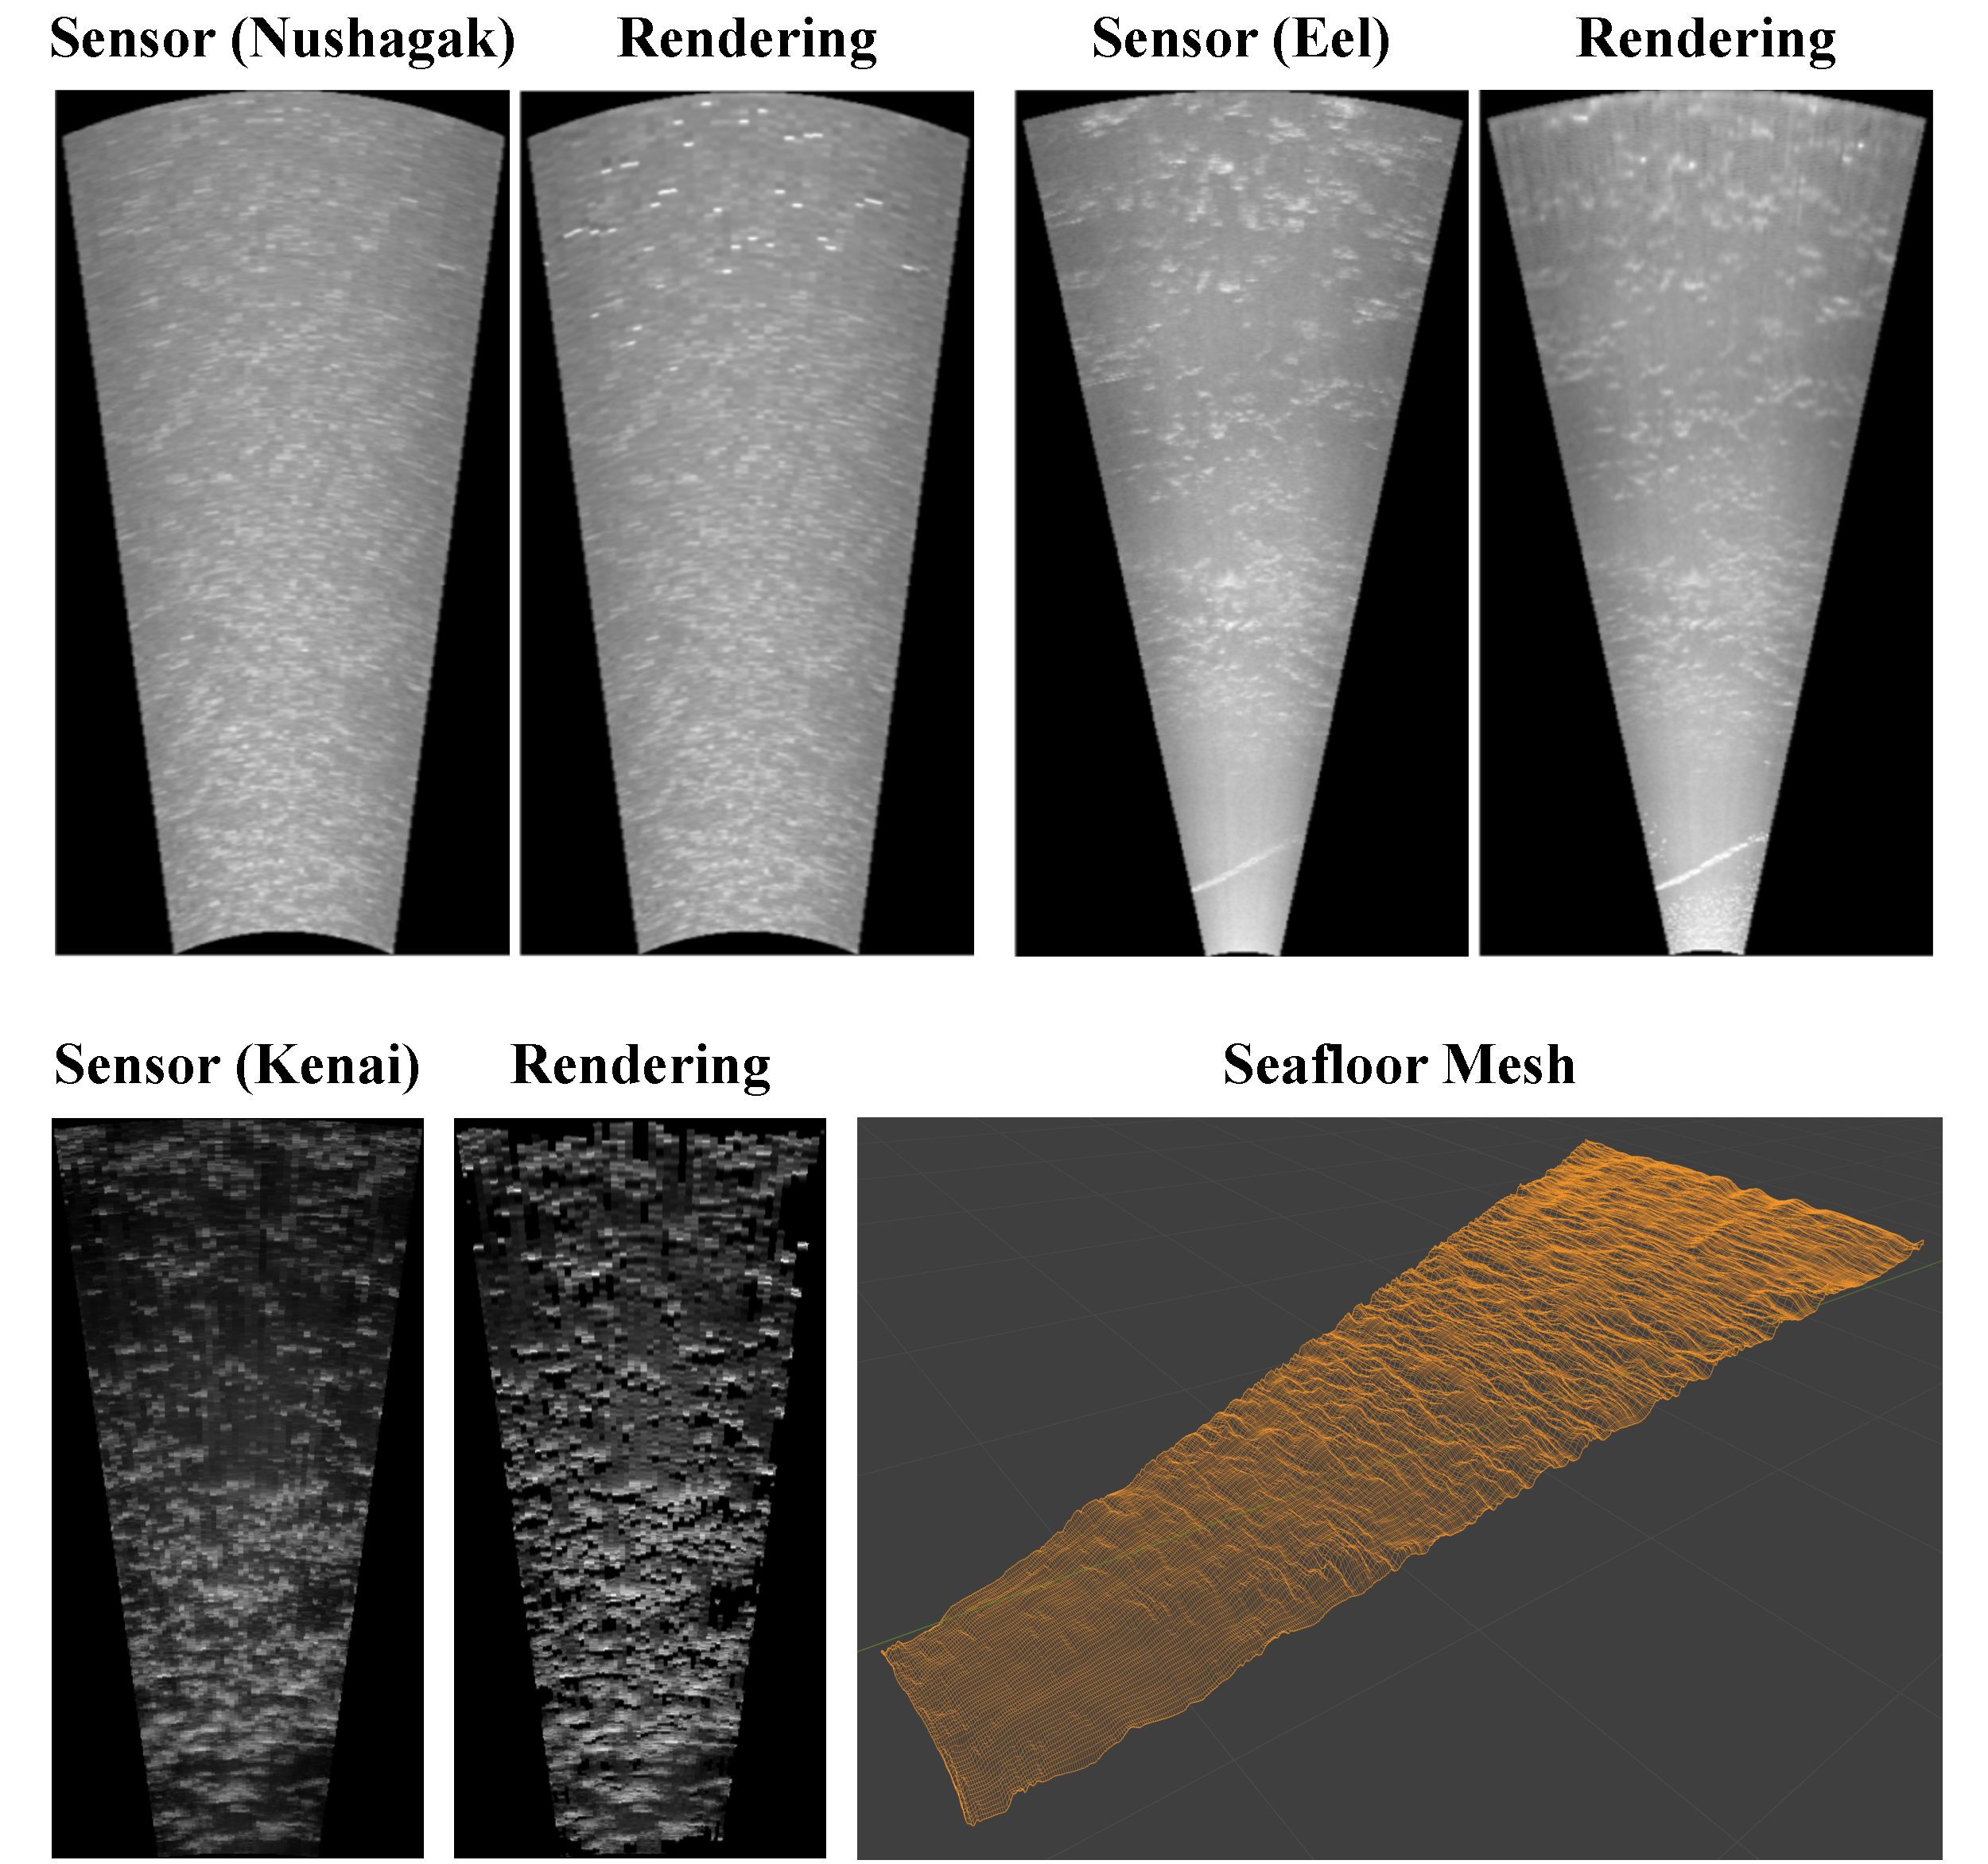
\includegraphics[width=1.0\columnwidth]{figs/river_fits.pdf}
  \caption{{\bf Sensor readings and reconstructed images using sonar images from real rivers} (\textit{cf.} Sec.~\ref{sec:qualitative}). From top-left to bottom are the Nushagak, Eel, and Kenai rivers. Additional 3D reconstructions are displayed in the supp. materials.}
  \label{fig:river_fits}
\end{figure}
\subsection{Failure Cases and Limitations}
\label{sec:limitations}

The primary limitation of our model lies in the inherent ambiguity present in single-view sonar imagery: many different geometries can explain the same observed sensor reading. In particular, our inverse renderer can achieve accurate recovery of geometric patterns, but tends to predict the minimum heights necessary to explain the observed data. Compared to a CNN, which can learn that occluded regions tend to have a certain depth, the height field gradients in our approach go to zero as the 2D image reconstruction approaches the target. This is both a strength and a limitation in our approach, since the differentiable renderer makes only the necessary geometric changes to explain observed data rather than relying on learned assumptions. We show this limitation explicitly in Fig.~\ref{fig:fail_case}, where we demonstrate a failure to recover the underlying heights even though the sensor reading is recovered accurately.

An additional limitation present in our differentiable renderer is that noise and artifacts in a target are explained by changes to the predicted geometry since we are optimizing for minimal reconstruction loss. This appears as high-frequency jumps in our predicted heights, which our TV regularization helps to reduce but doesn't fully eliminate.

\begin{figure}
  \centering
  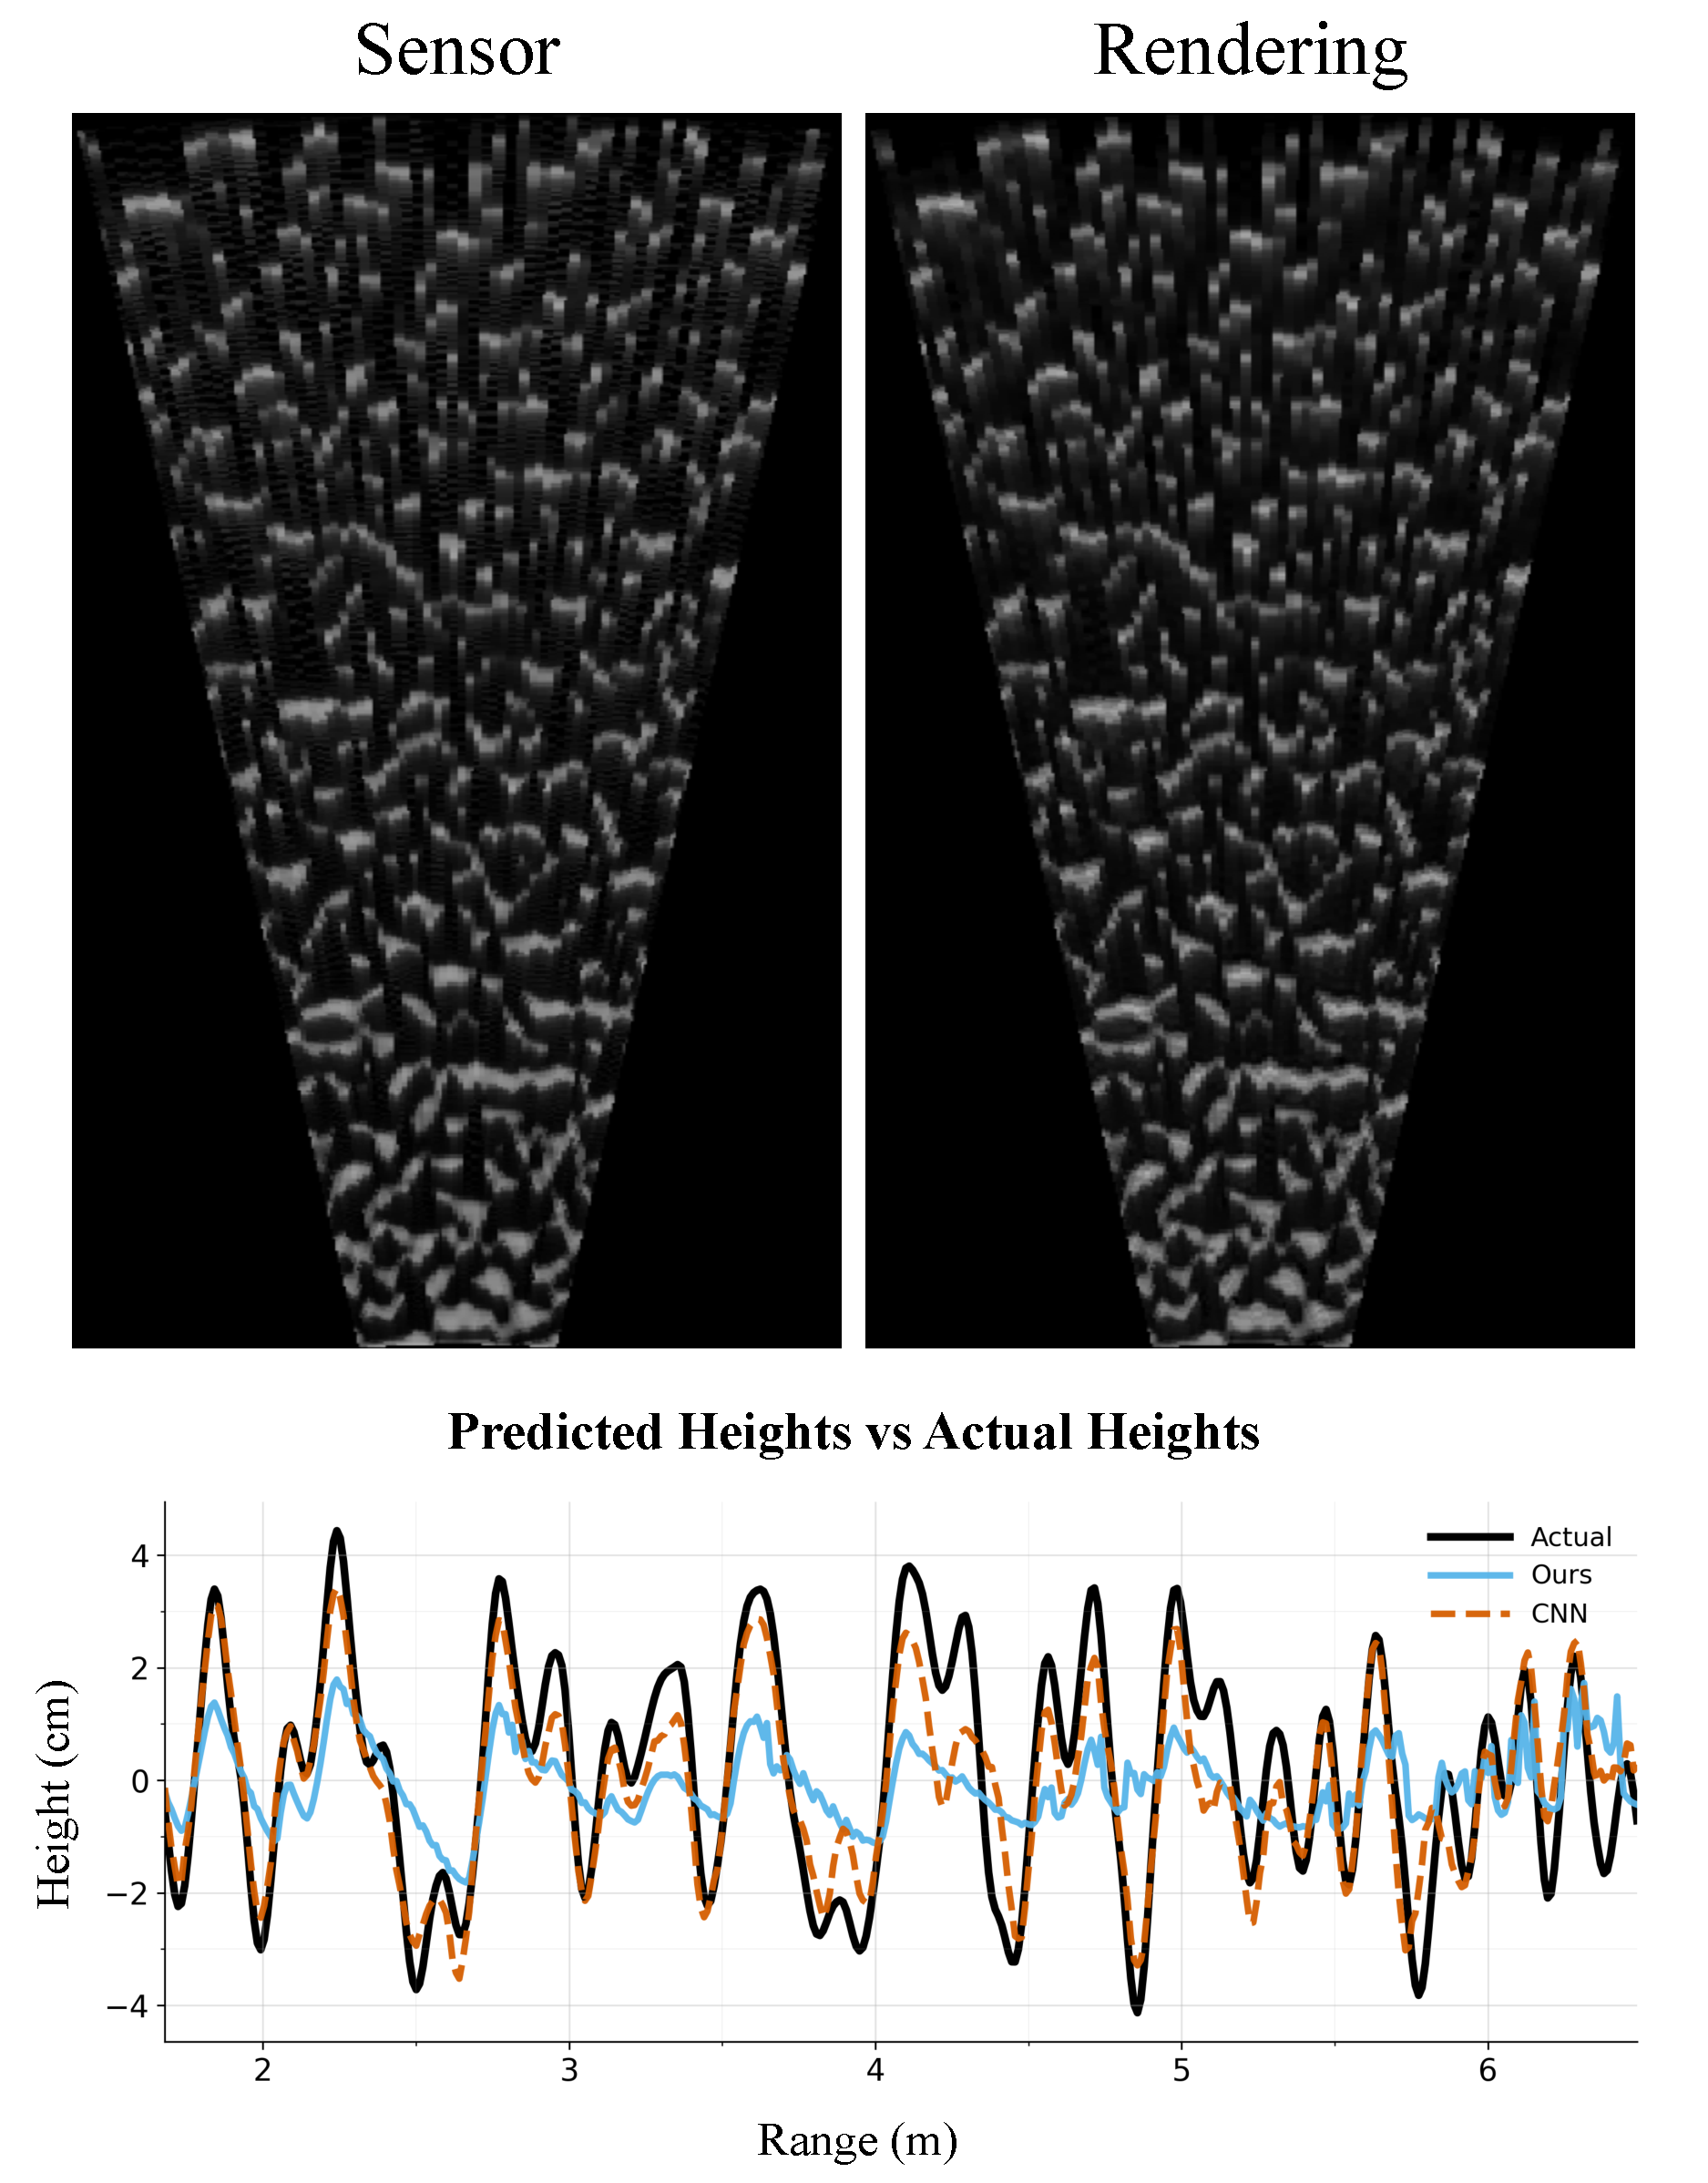
\includegraphics[width=0.85\columnwidth]{figs/fail_case.pdf}
  \vspace{-0.05in}
  \caption{{\bf Severe single-view ambiguities in imaging sonar}. Despite accurately reconstructing the sensor readings, this in-dist. sample's recovered heights are substantially shorter than the ground truth, as discussed in \cref{sec:limitations}. The CNN resolves this by learning the statistics of seafloor depth, and performs well.}
  \label{fig:fail_case}
  \vspace{-2mm}
\end{figure}

\subsection{TV Ablation}

We perform an ablation over \(\lambda_\text{TV}\) under the generic-view (GV) setting (Table~\ref{tab:tv_ablation}). Our method remains competitive across small values, but the results clearly benefit from a moderate smoothness prior that suppresses high-frequency artifacts. For our tasks, the best performance occurs with \(\lambda_\text{TV}\!=\!0.01\) on the in-distribution dataset, and around \(1.0\) on the standard HoloOcean and rough-terrain benchmarks.

\begin{table}[t]
  \centering
  \caption{
    \centering
    Increasing the TV regularization increases the accuracy of our method on HoloOcean. Evaluated using the generic viewpoint method and 3D MSE (cm, ↓).}
  \label{tab:tv_ablation}
  \begin{tabular}{lcccc}
    \toprule
    \(\lambda_\text{TV}\) & In Dist. & HoloOcean & HO Rough \\
    \midrule
    0 & {0.577} & 0.930 & 4.246 \\
    1e-2 & \textbf{0.575} & 0.923 & 4.244 \\
    1e-1 & {0.578} & {0.902} & {4.200} \\
    1.0 & 0.633 & \textbf{0.880} & \textbf{4.170} \\
    1e1 & 0.913 & 1.172 & 5.175 \\
    1e2 & 1.280 & 1.657 & 7.245 \\
    \bottomrule
  \end{tabular}
  \vspace{-3mm}
\end{table}
